\section{Fresnel zones}\label{sec:fresnel}
Taking into account that the application at hand involves radio communication, it is important to mention Fresnel zones. The Fresnel zone is the area around the visual line-of-sight where radio waves spread out into ellipse shaped areas when they leave the antenna. Thus, in Figure \ref{fig:3fresnel_zones} three Fresnel zones are stretched between two antennas, but actually there are an infinite number of them.

\begin{figure}[H]
	\centering
	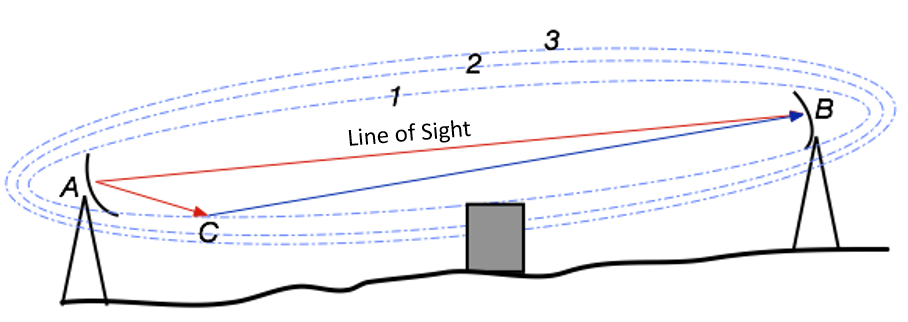
\includegraphics[scale=0.65]{figures/fresnel_zones.png}
	\caption{Fresnel zones between transmitter and receiver.}
	\label{fig:3fresnel_zones}
\end{figure}

The first zone is the one that has the most effect on the performance of the wireless network system. Thus, if there are any obstructions, such as buildings, trees or hills, in the first Fresnel zone, the signal will be affected by them and, consequently, it will be weaker at the receiver at both ends.

Therefore, it is essential to keep the first Fresnel zone clear of obstruction when planning wireless links. However, it is hard to avoid 100$\%$ of the obstructions in the real-life. Thus, based on, at least 60 $\%$ of the signal should be clear of obstructions. However, to get optimum performance it is recommended to have the obstructed signal less than 20$\%$ \cite{proxim}\cite{fresnelWiki}.

\subsection*{Fresnel zone calculations}
Figure \ref{fig:fresnel_zones} illustrates the first Fresnel zone between the antennas on buildings A and B. Thus, the radius, \textit{r}, corresponds to the radius of the Fresnel zone at point P. 

\begin{figure}[H]
	\centering
	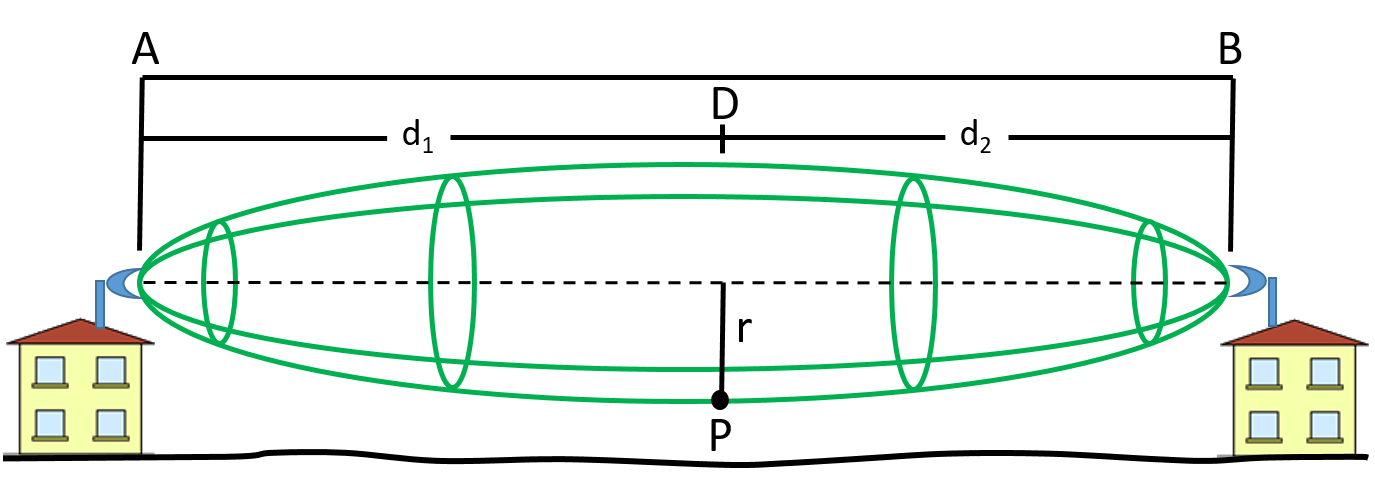
\includegraphics[scale=0.60]{figures/fresnel_zone.png}
	\caption{Fresnel zones diagram.}
	\label{fig:fresnel_zones}
\end{figure} 

Using Equation \ref{fresnel_zone_cal}, it is possible to calculate the radius, $r_n$, which represents the nth Fresnel zone at any point P and it depends on the wavelength of the transmitted signal, $\lambda$ \cite{fresnelWiki}. Thus, $d_1$ and $d_2$ represent the distances between the point P and the antennas A and B, respectively, in Figure \ref{fig:fresnel_zones}.

\begin{align}
r_n = \sqrt{\frac{n \lambda d_1 d_2}{d_1+d_2}} \label{fresnel_zone_cal}
\end{align}

On the other hand, it is often useful to know the maximum radius of the zone. The radius of the Fresnel zone achieves its maximum when both distances $d_1$ and $d_2$ have the same size ($d_1=d_2$, which means that $d_1+d_2=D$). Based on the relation between wavelength and frequency, $\lambda = \frac{c}{f}$, and on Equation \ref{fresnel_zone_cal}, the radius of the first Fresnel zone can be calculated using Equation \ref{eq:fresnel_radius3}. In this equation for ease of computation, the frequency, $f$, is taken in gigahertz(GHz), and the total distance between antennas, $D$, is in kilometres(km), thus, resulting the radius, $r$, in metres(m). 

\begin{align}
r_1 = \sqrt{\frac{c}{f}\frac{d_1 d_2}{d_1+d_2}} \stackrel{d_1=d_2=d}{=} \sqrt{\frac{c}{f}\frac{d^2}{2d}},  \label{eq:fresnel_radius1}
\end{align}

\begin{align}
r_1 = \sqrt{\frac{c}{2}}\sqrt{\frac{d}{f}} \stackrel{d=\frac{D}{2}}{=} \sqrt{\frac{c}{4}}\sqrt{\frac{D}{f}} \label{eq:fresnel_radius2}
\end{align}

\begin{align}
r_1 = 8.657 \sqrt{\frac{D}{f}} \label{eq:fresnel_radius3}
\end{align}

\subsection*{Fresnel Zones examples without curvature of the Earth}
Given Equation \ref{eq:fresnel_radius3} and changing the distance, D, three examples are shown in order to analyze the behaviour of the Fresnel zone radius' size, r. Thus, in the following examples, a frequency of 2.4 GHz is used but the curvature of the Earth is not considered. 

The first example shows the antennas of the GS and UA at a height of 20 and 100 meters, respectively, and a distance of 10km between them.

\begin{figure}[H]
	\centering
	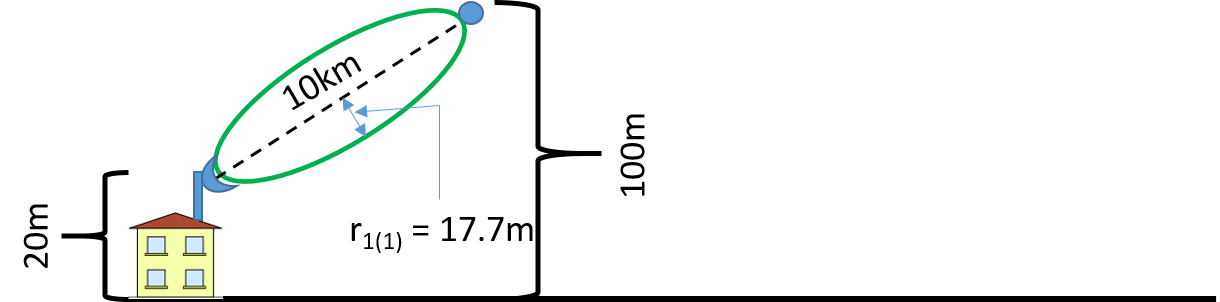
\includegraphics[scale=0.50]{figures/fresnel_10km.png}
	\caption{Fresnel zone. Calculations with 10km distance.}
	\label{fig:fresnel_zones_10km}
\end{figure}  

In this first example, the calculated radius is:
\begin{align*}
r_{1(1)} = 8.657 \sqrt{\frac{10}{2.4}} = 17.7m
\end{align*}

In the second example, the antennas are kept at the same heights as before, but the distance between them is 20km.

\begin{figure}[H]
	\centering
	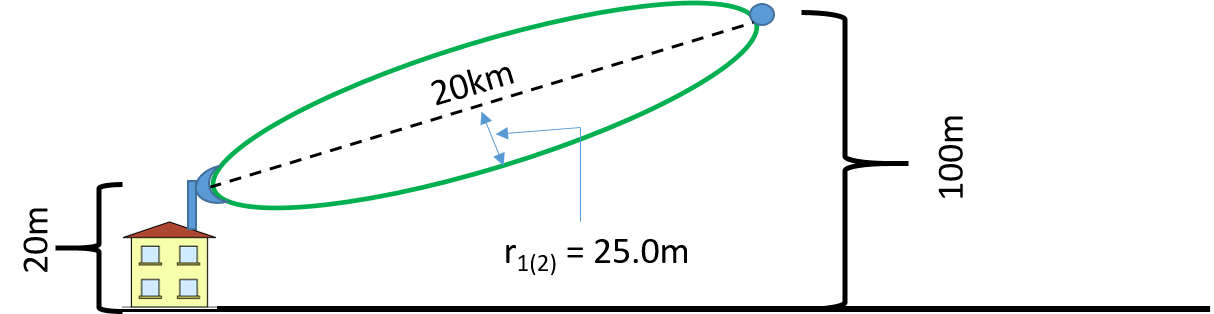
\includegraphics[scale=0.50]{figures/fresnel_20km.png}
	\caption{Fresnel zone. Calculations with 20km distance.}
	\label{fig:fresnel_zones_20km}
\end{figure}  

For this second example, the calculated radius is:
\begin{align*}
r_{1(2)} = 8.657 \sqrt{\frac{20}{2.4}} = 25.0m
\end{align*}

In the last example, the GS and UA antennas kept at the same heights as in the previous examples, but the distance between them is 50km.

\begin{figure}[H]
	\centering
	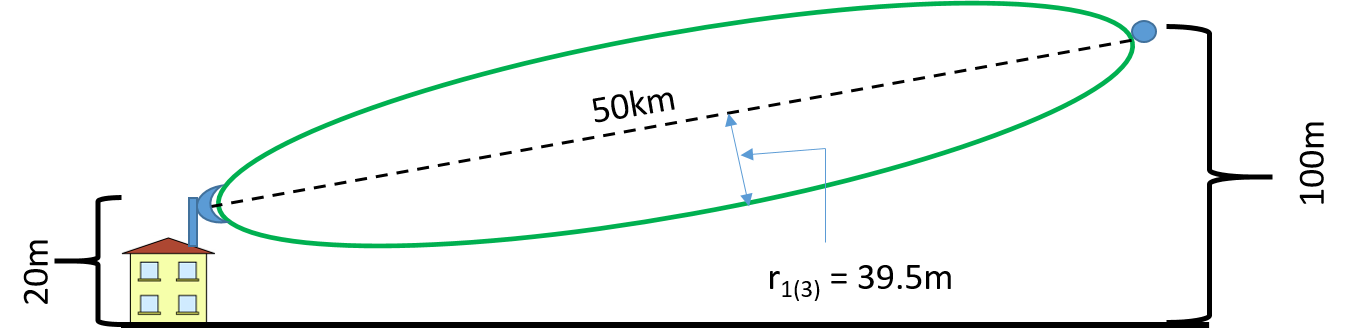
\includegraphics[scale=0.50]{figures/fresnel_50km.png}
	\caption{Fresnel zone. Calculations with 50km distance.}
	\label{fig:fresnel_zones_50km}
\end{figure}  

In the last case, the calculated radius is:
\begin{align*}
r_{1(3)} = 8.657\sqrt{\frac{50}{2.4}} = 39.5m
\end{align*}

After these examples it can be seen that the radius of the Fresnel zone increases when the distance between the antennas increase.

\subsection*{60$\%$ Clearance Zone of the first Fresnel zone}
As it was described in the beginning of this section, it is difficult to have a first Fresnel zone without any obstructions. However, a percentage of obstruction equal or smaller than 40$\%$ makes the connection possible between the transmitter and the receiver.

In this subsection, some examples will demonstrate how tall an obstruction can be at the center of the first Fresnel zone, taking into account the 60$\%$ clearance. These calculations were made with the help of Equation \ref{eq:60_percent_radius}, which resulted from Equation \ref{eq:fresnel_radius3} by multiplying it with the clearance factor of 60$\%$ \cite{viasFresnel}.

\begin{align}
r_1 = 8.657\sqrt{0.6\frac{D}{f}}\label{eq:60_percent_radius}
\end{align}

For an ideal case, assuming that both antennas are at a height of 20 meters (operating at 2.4GHz) and the distance between them is 10km, the radius is given by Equation \ref{eq:100_distance10}.

\begin{align}
r_1 = 8.657\sqrt{\frac{10}{2.4}} = 17.7m\label{eq:100_distance10}
\end{align}

In this case, the first Fresnel zone would pass just 2.3 meters above the ground level in the middle of the link. 

\begin{figure}[H]
	\centering
	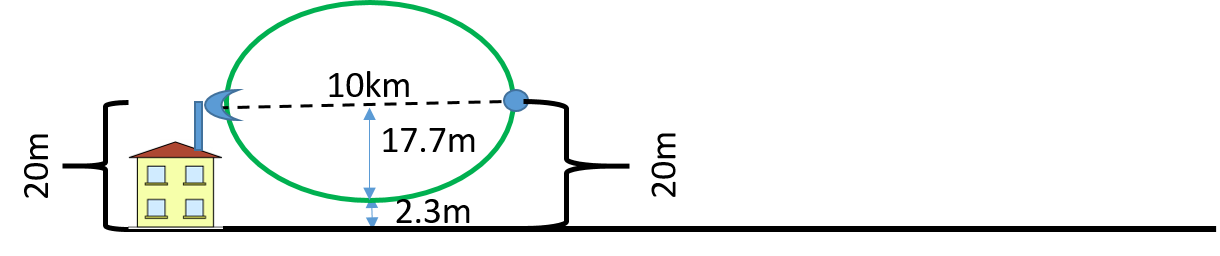
\includegraphics[scale=0.50]{figures/fresnel_10km_height.png}
	\caption{Fresnel zone. Antennas at same height and 10km distance.}
	\label{fig:fresnel_zones_10km_height}
\end{figure}  

In order to calculate how tall a structure should be, it is necessary to calculate the radius of the Fresnel zone when the signal is 60$\%$ cleared (Equation \ref{eq:60_distance10}).

\begin{align}
r_{1(60\%)} = 8.657\sqrt{0.6 \frac{10}{2.4}} = 13.7m\label{eq:60_distance10}
\end{align}
  
Therefore, knowing that the height of the longitudinal axis of the ellipsoid is the same as the one of both antennas, it is possible to calculate the maximum altitude of the obstruction. This altitude can be obtained by subtracting the antenna height with the radius calculated in Equation \ref{eq:60_distance10}.

\begin{align}
\text{$O_{h,max}$} = 20 - 13.7 = 6.3m\label{eq:height_obstruction}
\end{align}

Hence, for this specific example, the maximum tolerated height of any obstruction located in the middle point between both antennas is 6.3m. An illustration of this situation is shown in Figure \ref{fig:fresnel_zones_10km_60procent}.

\begin{figure}[H]
	\centering
	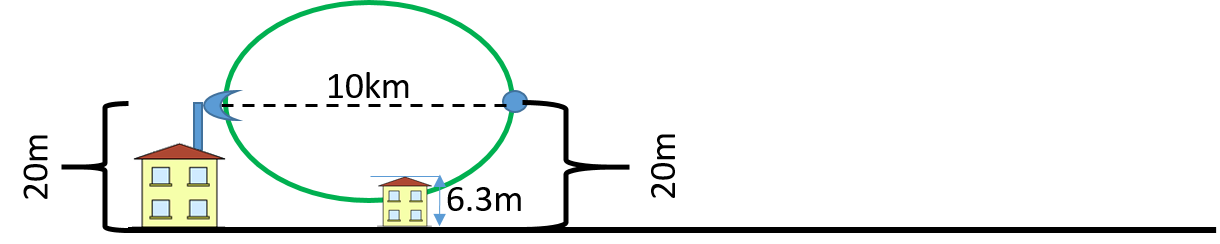
\includegraphics[scale=0.50]{figures/fresnel_10km_60procent.png}
	\caption{Fresnel zone with a 40$\%$ of blocked signal.}
	\label{fig:fresnel_zones_10km_60procent}
\end{figure}  

An obstruction higher than 6.3m will give less than 60$\%$ clearance of the Fresnel zone. To prevent this problem, the antenna could be positioned higher, the frequency could be changed or the direction of the link should be changed to avoid obstacles.

\subsection*{Fresnel zones examples with curvature of the Earth}
For longer distance links the curvature of the Earth comes into play and it may result in obstruction of the Fresnel zone, causing signal losses. Moreover, the longer the distance between the antennas, the greater the radius of the Fresnel zone. Equation \ref{eartheffect} helps compute the height difference of the Earth's curvature, $H$, at the mid-point between the two antennas  \cite{4Gonsolution}. In order to do the previous calculation, it is necessary to include one parameter related to the total distance between both antennas, $D$ (km), and one related to the effective radius of Earth, $E_r = 8 504 km$.

Furthermore, Figure \ref{fig:fresnel_50km_curvature} is an illustration where the curvature of the Earth is taken into account. On this Figure the antennas on the GS and the UA are at a 77m height and the distance between them is 50km. 

\begin{align}
H [m] = \frac{1000\cdot D^2}{8\cdot E_r}\label{eartheffect}
\end{align}

\begin{figure}[H]
	\centering
	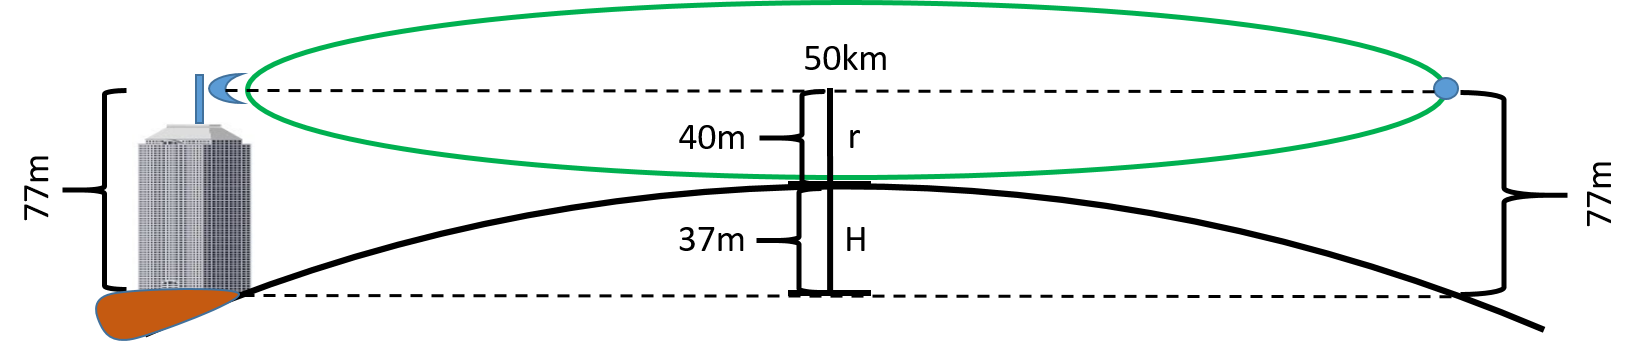
\includegraphics[scale=0.50]{figures/fresnel_50km_curvature.png}
	\caption{Fresnel zone with 50km distance. Calculations on the Earth's surface.}
	\label{fig:fresnel_50km_curvature}
\end{figure}

Based on Equation \ref{eartheffect}, the height difference of the Earth's curvature at the mid-point between the UA and GS \cite{4Gonsolution}:
\begin{align}
\text{H} = \frac{1000 D^2}{8 \cdot E_r} = \frac{1000 \cdot 50^2}{8\cdot 8504} = 36.7m \approx 37m 
\end{align}

Furthermore, the radius of the first Fresnel zone:
\begin{align*}
\text{r} = 8.657\cdot \sqrt{0.6\cdot\frac{D}{f}} = 8.657\cdot \sqrt{0.6\cdot\frac{50}{2.4}} = 39.5m \approx 40m 
\end{align*}

On the other hand, the maximum height of the obstruction between the two devices within the 60$\%$ clearance zone can be calculated with the Equations \ref{radius_60}, \ref{Obs_max_height} and \ref{height_max_with_curv}. These calculations are illustrated on Figure \ref{fig:fresnel_50km_curvature_obstacle}.

\begin{align}
r_{1(60\%)} &= 8.657\cdot \sqrt{0.6\cdot\frac{D}{f}} = 8.657\cdot \sqrt{0.6\cdot\frac{50}{2.4}} = 30.6m \approx 31m \label{radius_60}
\end{align}

The maximum height of the obstruction and the curvature of the Earth included:
\begin{align}
\text{OC}_{\text{h,max}} &= 77m - r_{1(60\%)} = 77m - 31m = 46m \label{Obs_max_height}
\end{align}

The actual maximum height of the obstruction:
\begin{align}
\text{O}_{\text{h,max}} &= \text{OC}_{\text{h,max}} - H = 46m - 37m = 9m
\label{height_max_with_curv}
\end{align}

\begin{figure}[H]
	\centering
	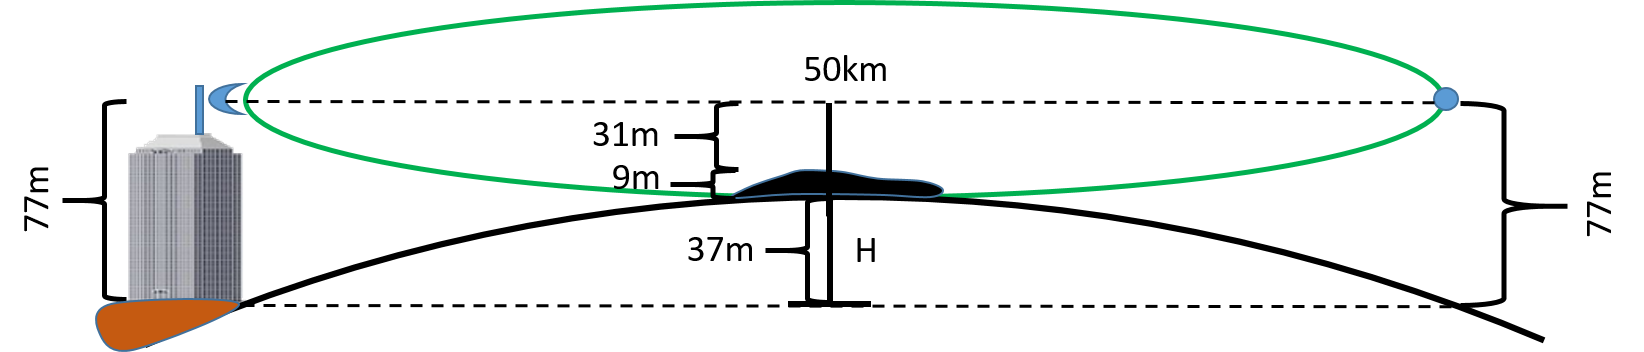
\includegraphics[scale=0.50]{figures/fresnel_50km_curvature_obstacle.png}
	\caption{Fresnel zone with 50km distance. Calculations on the Earth's surface with 60$\%$ clearance.}
	\label{fig:fresnel_50km_curvature_obstacle}
\end{figure}  

Figure \ref{fig:fresnel_50km_curvature_obstacle} shows how important it is to consider the curvature of the Earth. In this case, the obstruction can only be at a height of 9m, since the curvature is an obstruction itself and takes 37m. However, it is important to note that this example only implies when the longitudinal axis of the ellipsoid is the same as the one of both antennas. But nonetheless it gives a good understanding that the Fresnel zones are important factors when building a wireless link network.
